\section{Literature Review}
\subsection{Fuel Cell Operation, Subsystems and Parameters}
\paragraph{}In a (Proton Electron Membrane)PEM fuel cell stack, chemical energy from the reaction between hydrogen and oxygen is converted directly into electric energy. Water and heat are produced as by-products \cite{thanapalan_model_2011}.
\begin{figure}[!h]
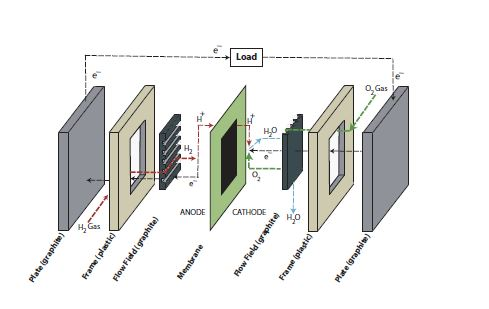
\includegraphics{Figures/Figure5}
\caption{Fuel cell component description
\cite{stefanopoulou_mechatronics_nodate}}
\end{figure} 
\paragraph{}In a hydrogen fuel cell, hydrogen (which we will also refer to as fuel) travels through inlet manifolds to the flow fields. From the flow fields, gas diffuses through porous media to the membrane. The membrane, which is sandwiched in the middle of the cell, contains catalyst and microporous diffusion layers along with gaskets as a single integrated unit. One side of the membrane is  the anode and the other is the cathode. The anode and cathode are more generally referred to as electrodes. The catalyst layer at the anode separates hydrogen molecules into protons and electrons \cite{stefanopoulou_mechatronics_nodate}.
\begin{equation}
$$2H_{2} \rightarrow 4H^{+}+4e^{-}$$
\end{equation}
\paragraph{}The membrane permits only the transfer of  hydrogen protons, requiring the electrons to flow through an external circuit before recombining with protons and oxygen at the cathode-to form water.
\begin{equation}
$$O_{2}+H^{+} + 4e^{-}\rightarrow 2H_{2}O $$
\end{equation}
\paragraph{}The migration of electrons produces electricity. The overall reaction of the fuel cell is:
\begin{equation}
$$2H_{2}+ O_{2} \rightarrow 2H_{2}O+Heat.$$
\end{equation}
\paragraph{}The electrical characteristics of fuel cells are given in the form of a polarization curve, shown in Figure 2.2 , which is a plot of cell voltage versus cell current density (current per unit cell active area) at different reactant pressures and flows.
\begin{figure}[!h]
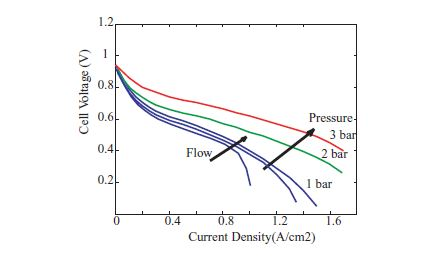
\includegraphics{Figures/Figure6}
\caption{Fuel cell component description
\cite{stefanopoulou_mechatronics_nodate}}
\end{figure}
\paragraph{}Stack temperature and membrane water content affect the fuel cell voltage \cite{ehsani_modern_2018}. The difference between the actual voltage and the ideal voltage represents the loss in the cell which turns into heat. (The ideal standard voltage for a fuel cell in which H2 and O2 react is 1.18 V when the resulting water product is in gaseous form.)
\paragraph{}As more current is drawn from the fuel cell, the voltage decreases, due to fuel cell electrical resistance, low reaction rate and, inefficient reactant gas transport,. Lower voltage indicates lower efficiency of the fuel cell, therefore low load (low current) operation is preferred. Operation at low load requires a large fuel cell stack and has detrimental consequences to the overall volume, weight, and cost.
\paragraph{}To avoid over-sizing the FC stack, a series of actuators such as valves, pumps, blowers, expander vanes, fan motors, humidifiers and condensers are used to control critical FC parameters for a wide range of current, and thus, power setpoints. The auxiliary actuators are needed to make fine and fast adjustments to satisfy reliability standards, performance and safety that are independent of age and operating conditions of the FC. The resulting multivariate design and control synthesis task, also known as balance of plant (BOP), is complex because of subsystem interactions, conflicting objectives, and lack of sensors.
\paragraph{}Main Control among the main FC subsystems are:
\begin{itemize}
\item reactant supply system
\item heating and cooling system
\item humidification system
\item Power management System
\end{itemize}
\paragraph{}The main control variables in FC systems are: 
\begin{itemize}
\item Stack temperature
\item Membrane humidity
\item Accumulation of water and nitrogen in the anode side. 
\end{itemize}
\paragraph{}These variables are the most important factors for any efficiency and lifetime of FC stacks.
\paragraph{}Previous research has concluded that since the fuel cell is a passive power source, a simple feed forward control strategy is used to control the air supply and A PI-feedback algorithm is developed to control the cooling water temperature. The research further concludes that the control strategies need to be further optimized basing on a nonlinear dynamic model.
\begin{figure}[!h]
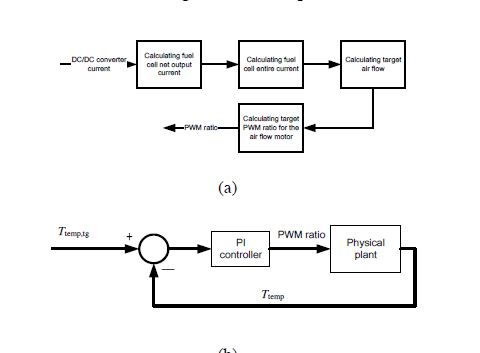
\includegraphics{Figures/Figure8}
\caption{Fuel cell control strategy (a) the air supply system (b) the heat management system
\cite{xu_hierarchical_2010}}
\end{figure}

\paragraph{}Dr. J.T. Pukrushpan et al.\cite{pukrushpan_modeling_2003} studied modelling and control for PEM fuel cell stack
systems, and published several papers. They proposed a nonlinear dynamic model to describe
the PEM fuel cell system, and designed feedback controllers based on the model.
\paragraph{}Further, there have been efforts devoted in controlling the reactant flow system in PEMFCs using only voltage and current measurements and inferring power. More specifically, a single-input
single-output (SISO) controller between the compressor motor voltage and the delivered current or power to the traction motor. Temperature control in available systems is done using large radiators. As a control mechanism to prevent anode flooding, various ingenious mechatronic solutions have been proposed to abate anode flooding (Rodatz et al., 2002)
 \cite{stefanopoulou_mechatronics_nodate}.
\subsection{Fuel Cell Control}
\begin{figure}[!h]
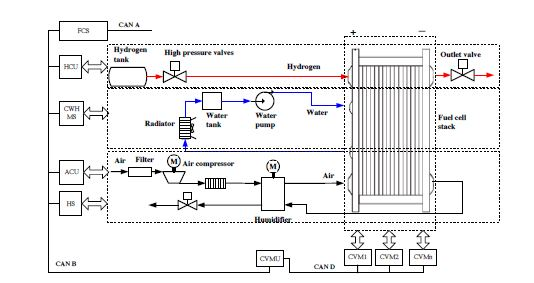
\includegraphics{Figures/Figure7}
\caption{Hydrogen Fuel Cell Control
\cite{xu_hierarchical_2010}}
\end{figure}
\paragraph{}The Fuel cell consists of a hydrogen supply system, a water and heat management system and an air supply system. The compressed hydrogen is stored in several tanks, under  pressures of about 30 MPa. The hydrogen pressure is lowered and kept at a stable level using several valves for safety purposes before the hydrogen goes into the stack. Water accumulates in the stack due to the electrochemical reaction during the operation of the fuel cell, which leads to performance decay. An outlet valve is installed so that the accumulated water can be blown away with hydrogen. The outlet valve and the hydrogen valves used for lowering and stabilizing the pressure are controlled by the Hydrogen Control Unit (HCU).
\paragraph{}The electro-chemical reaction also generates heat, and causes the temperature to increase. The water and heat management system targets to control the stack temperature within a suitable range using deionized water in a water tank. The water flow is controlled by a water pump. The water goes into the stack with a low temperature, and comes out of the stack with a high temperature. A radiator is used to cool the warm water.
\paragraph{}The cooling water temperature is measured, and controlled by a feedback control algorithm.
The air supply system comprises an air filter, a compressor and a humidifier. The impurities in air will cause the catalyst to be poisoned. Thus as a preventive measure, the air should be filtered before getting into the stack. The air flow is controlled by the compressor with a feed forward + feedback algorithm. 
\paragraph{}The air is further humified since there should be some water in the PEM, to allow the PEM to conduct protons. In the humidifier, the dry air is humidified with the damp-heat air out of the stack. The air compressor and the humidifier are controlled by the Air Control Unit (ACU) and the Humidifying System (HS).
\subsection{Summary}
\paragraph{}A fuel cell system integrates many components into a power system. These include DC/DC converters, batteries, and ultracapacitors in the system. In cases where the fuel cell is not fed directly with hydrogen, a reformer must be included. Therefore, there are many control loop schemes, the number of which depends on the configuration of the system. 
\paragraph{}Many control strategies have been proposed in literature, ranging from feed-forward control,Linear quartertic regulator, Neural Networks and Model Predictive Control. A good number of research papers focus on the low level control of the fuel cell to fulfil at least one of the three main objectives such as maximum efficiency, voltage control and/or starvation prevention. However, these designs are still at the theoretical stage and without real time testing. This leads to a methodological gap in the area of hydrogen fuel cell control. The validity of these control strategies for real fuel cell system applications is, however, still under investigation. 
\paragraph{}Furthermore, the extensive studies in the controller design methods are evidence that the fuel cell system control is a very active research area. The research in this area is mainly motivated by the recognition that the current control methods cannot fully meet the desired design requirements on fuel cell system performance, stability, and robustness etc. Any controller design which gives a satisfactory performance on fuel cell system behavior is worth consideration for implementation \cite{ehsani_modern_2018}.

